%!TEX root = ../dissertation.tex
\chapter{Introduzione}
\label{introduzione}

Il recupero e la classificazione di forme 3D sono stati oggetto di una grande quantità di lavori di ricerca che sfruttano sia la rappresentazione globale che i descrittori di forma locale. Un panoramica del campo può essere trovata in \cite{Tangelder2007}, \cite{YulanGuo2014}, \cite{BoYijuan} o guardando le varie edizioni del SHREC 3D Retrieval Contest \cite{ShrecContest}. 

Questo progetto si focalizza sul riconoscimento di gesti delle mani, ambito di notevole interesse dovuto alle sue applicazioni in molti campi diversi come l'interazione uomo-computer, la robotica, i giochi per computer e l'interpretazione automatica della lingua dei segni.
I recenti conseguimenti nel campo della Computer Vision hanno permesso di ottenere un miglioramento notevole in algoritmi di questo tipo. In particolare ci sono stati due avanzamenti chiave:

\begin{itemize}
\item Sviluppo di algoritmi di machine learning più potenti, specialmente tecniche di deep learning.
\item Introduzione di telecamere di profondità, come Time-Of-Flight e Structured-light cameras \cite{DalMutto2012}.
\end{itemize}

La soluzione del problema di classificazione di forme 3D usando dati di immagini e video è sempre stata molto impegnativa, ma lo sviluppo di questi due campi ha permesso, sia di capire meglio il contenuto semantico delle immagini, che di utilizzare approcci basati su informazioni tridimensionali. Ad esempio i dati di profondità che si riescono ad ottenere da queste telecamere contengono una descrizione molto accurata della posa della mano e questo è molto utile per le applicazioni di riconoscimento dei gesti.
Il progetto si basa sullo studio di 5 approcci differenti che combinano diverse architetture della rete e vari tipi di dati di input. Infatti non ci si sofferma solo su dati di profondità ma si utilizzano anche mappe di confidenza e immagini RGB. L'unione di queste informazioni porta ai risultati presentati consultabili nelle tabelle alla fine del Capitolo \textbf{\ref{Risultati sperimentali}}.\\

Questa tesi è composta da una parte introduttiva riguardante le Deep Neural Networks e i suoi algoritmi di ottimizzazione, una parte centrale che illustra il set di dati utilizzato e le sue elaborazioni, successivamente vengono spiegate diverse architetture della Convolutional Neural Network utilizzata per il riconoscimento di 11 gesti differenti, ed infine una parte conclusiva di analisi dei risultati.\\

\begin{comment}
Le reti neurali sono basate su tipi di neuroni artificiali. Il primo di essi venne sviluppato negli anni '50 e '60 ed fu chiamato Perceptron. Oggi, è più comune usare altri modelli di neuroni artificiali, ad esempio quello proposto in questo progetto: il Sigmoid Neuron.
Per capire meglio come funziona un Sigmoid Neuron bisogna però accennare al funzionamento di un Perceptron.
La rappresentazione accetta diversi input binari, x1, x2, … e produce una singola uscita binaria:

\begin{figure}
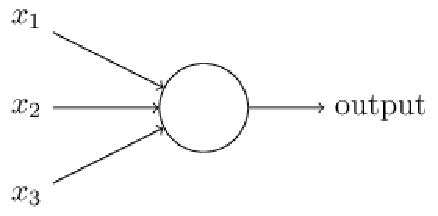
\includegraphics[width=%
0.5\textwidth]{figures/fig01}
\caption[Idea di un perceptron.]{Figura rappresentativa .
\label{fig:myInlineFigure}}
\end{figure}


Nell'esempio mostrato il perceptron ha tre ingressi, x1, x2, x3. In generale potrebbe avere più o meno input. Rosenblatt ha proposto una semplice regola per calcolare l'output. Ha introdotto pesi , w1, w2, … numeri reali che esprimono l'importanza dei rispettivi input per l'output. L'uscita del neurone, 0 o 1, è determinato dal fatto che la somma ponderata ΣjwjXj è minore o maggiore di qualche valore di soglia ( threshold value ). Proprio come i pesi, la soglia è un numero reale che è un parametro del neurone. Per metterlo in termini algebrici più precisi:

$$Output =
\bigg \{
\begin{array}{rl}
0 & \sum_j ( j \, w_j \, X_j ) \le threshold \\
1 & \sum_j ( j \, w_j \, X_j ) > threshold \\
\end{array}
$$

Questo è il modello matematico di base. Un modo in cui puoi pensare al perceptron è che è un dispositivo che prende le decisioni soppesando le prove e da cui, variando i pesi e la soglia, possiamo ottenere diversi modelli di decisione.

Per inciso, quando ho definito i perceptrons ho detto che un perceptron ha solo una singola uscita. Nella rete sopra i perceptron sembrano avere più uscite. In realtà, sono ancora a uscita singola. Le frecce di output multiple sono solo un modo utile per indicare che l'output di un perceptron viene utilizzato come input per molte altre percetron. È meno ingombrante del disegnare una singola linea di uscita che poi si divide.
Semplifichiamo il modo in cui descriviamo i peceptrons.
Il primo cambiamento è scrivere $\sum_j ( j \, w_j \, X_j )$ come prodotto, 
$ w \cdot x \equiv \sum_j ( j \, w_j \, X_j )$, dove w e x sono vettori i cui componenti sono rispettivamente i pesi e gli input. Il secondo cambiamento è spostare la soglia dall'altra parte della disuguaglianza e sostituirla con quella che è nota come bias del perceptron , $b \equiv -threshold$. Usando il bias invece della threshold, la formula del perceptron può essere riscritta:

$$Output =
\bigg \{
\begin{array}{rl}
0 & w\cdot X + b \le 0 \\
1 & w\cdot X + b > 0 \\
\end{array}
$$


Puoi pensare al bias come misura di quanto sia facile far percepire al perceptron un 1. O, per dirla in termini più biologici, la polarizzazione è una misura di quanto sia facile ottenere il perceptron a fuoco . Per un perceptron con una distorsione veramente grande, è estremamente facile per il perceptron emettere un 11. Ma se il bias è molto negativo, allora è difficile per il perceptrone emettere un 1. Ovviamente, introdurre il bias è solo un piccolo cambiamento nel modo in cui descriviamo i percetron, ma vedremo in seguito che questo porta a ulteriori semplificazioni notazionali. Per questo motivo, nel resto del libro non useremo la soglia, useremo sempre il bias.

Tuttavia, la situazione è migliore di quanto suggerisca questa visione. Si scopre che possiamo escogitare algoritmi di apprendimento in grado di sintonizzare automaticamente i pesi e le distorsioni di una rete di neuroni artificiali. Questa sintonizzazione avviene in risposta a stimoli esterni, senza l'intervento diretto di un programmatore.



\newthought{Sigmoid Neuron}

Per vedere come potrebbe funzionare l'apprendimento, supponiamo di fare un piccolo cambiamento in alcuni pesi (o bias) nella rete. Quello che vorremmo è che questo piccolo cambiamento di peso causi solo una piccola variazione corrispondente nell'output dalla rete. Come vedremo tra un momento, questa proprietà renderà possibile l'apprendimento. Schematicamente, ecco cosa vogliamo:

\begin{figure}
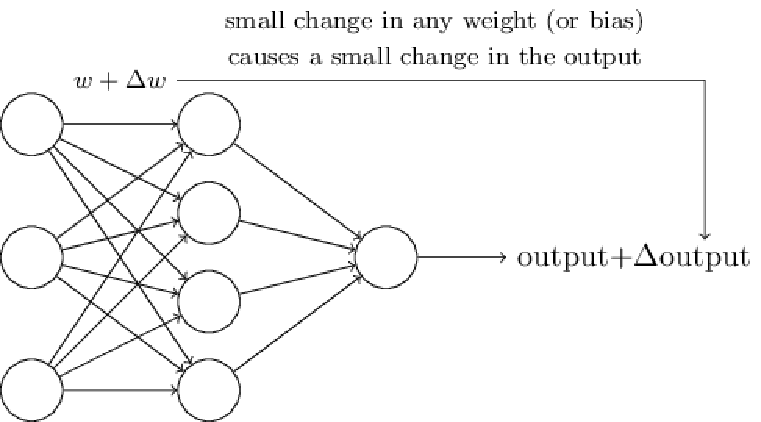
\includegraphics[width=%
0.8\textwidth]{figures/fig08}
\caption[Idea di un s.]{Figura rappresentativa .
\label{fig:myInlineFigure}}
\end{figure}

Se fosse vero che un piccolo cambiamento in un peso (o bias) causa solo un piccolo cambiamento nell'output, allora potremmo usare questo fatto per modificare i pesi e i bias per far sì che la nostra rete si comporti più nel modo che vogliamo. Poi lo ripetiamo, cambiando pesi e bias ripetutamente per produrre risultati migliori e migliori. La rete starebbe imparando.
Il problema è che questo non è ciò che accade quando la nostra rete contiene percetrons. In effetti, un piccolo cambiamento nei pesi o nei bias di ogni singolo perceptron nella rete può a volte far capovolgere completamente l'output di quel perceptron, diciamo da 0 a 1. Questo lancio potrebbe quindi far cambiare completamente il comportamento del resto della rete in un modo molto complicato. 
Ciò rende difficile vedere come modificare gradualmente i pesi e i bias in modo che la rete si avvicini al comportamento desiderato. Forse c'è un modo intelligente per aggirare questo problema. Ma non è immediatamente ovvio come possiamo ottenere una rete di percetrons da imparare.
Possiamo superare questo problema introducendo un nuovo tipo di neurone artificiale chiamato sigmoid neuron . I sigmoid neurons sono simili ai perceptrons, ma modificati in modo che piccoli cambiamenti nei loro pesi e bias causino solo un piccolo cambiamento nella loro produzione. Questo è il fatto cruciale che permetterà a una rete di sigmoid neurons di imparare. 
Descriveremo i sigmoid neurons nello stesso modo in cui abbiamo rappresentato i perceptrons:

Proprio come un perceptron, il sigmoid neuron ha input, x1, x2, … Ma invece di essere solo 0 o 1, questi input possono anche assumere qualsiasi valore compreso tra 0 e 1. Quindi, ad esempio, 0.638... è un input valido per un sigmoid neuron. Inoltre, proprio come un perceptron, il sigmoid neuron ha pesi per ogni input, w1, w2, … e un bias complessivo. Ma l'output non è 0 o 1. 
Invece, è σ ( w ⋅ x + b ), dove σ è chiamata la funzione sigmoide (sigmoid function) ed è definito da:\\

\begin{eqnarray} 
\sigma(z) \equiv \frac{1}{1 + e^{-z}}
\end{eqnarray}

Per dirla in modo un po' più esplicito, l'output di un sigmoid neuron con ingressi x1, x2, …, pesi w1, w2, … e bias b è : \\
\begin{eqnarray} 
\sigma(z) \equiv \frac{1}{1+\exp(-\sum_j w_j x_j-b)}
\end{eqnarray}


A prima vista, i sigmoid neurons appaiono molto diversi dai perceptrons. La forma algebrica della funzione sigmoide può sembrare opaca e proibitiva se non la conosci già. In effetti, ci sono molte somiglianze tra i perceptrons e i sigmoid neurons e la forma algebrica della funzione sigmoide risulta essere più un dettaglio tecnico che una vera barriera alla comprensione.
Per capire la somiglianza con il modello perceptron, supponiamo che 
$z \equiv  w \cdot x + b$ sia un grande numero positivo. Quindi $e^{-z} \approx 0$ e così $\sigma(z) \approx 1$.
In altre parole, quando $z= w \cdot x + b$ è grande e positivo, l'uscita dal sigmoid neuron è di circa 1, proprio come sarebbe stato per un perceptron. Supponiamo d'altra parte che $z = w \cdot x + b$ è molto negativo. Quindi $e^{-z} \to \infty$ e $\sigma(z) \approx 0$. Quindi, quando$ z= w \cdot x + b$ è molto negativo, anche il comportamento di un sigmoid neuron si avvicina molto a un perceptrons. È solo quando $z = w \cdot x + b$ è di dimensioni modeste che c'è molta deviazione dal modello perceptron.
Che dire della forma algebrica di $\sigma$? Come possiamo capirlo? In effetti, la forma esatta di σ non è così importante - ciò che conta davvero è la forma della funzione quando è tracciata. Ecco la forma:

\begin{figure}
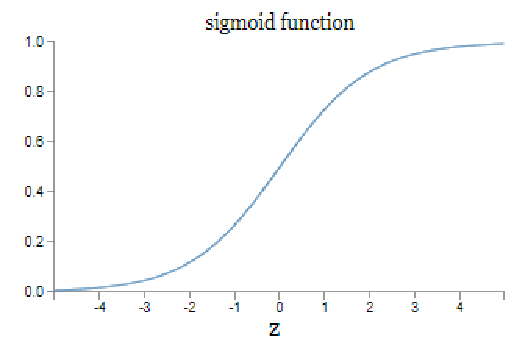
\includegraphics[width=%
0.8\textwidth]{figures/fig10}
\caption[Sigmoid function.]{Figura rappresentativa .
\label{fig:myInlineFigure}}
\end{figure}

Questa forma è una versione attenuata di una funzione di passaggio:

\begin{figure}
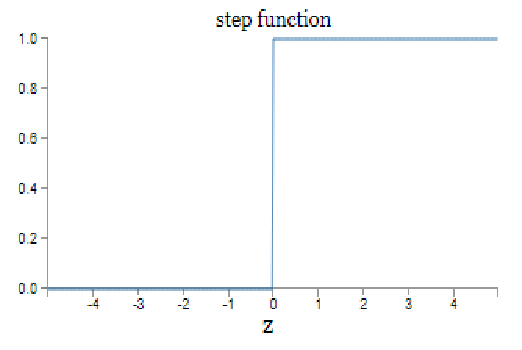
\includegraphics[width=%
0.8\textwidth]{figures/fig11}
\caption[Step function.]{Figura rappresentativa .
\label{fig:myInlineFigure}}
\end{figure}

Se σ era in effetti una funzione a gradino, allora il sigmoide sarebbe stato un perceptron, poiché l'output sarebbe 1 o 0 a seconda che w⋅x+b era positivo o negativo * . Usando il σ attuale la funzione che otteniamo, come già implicato sopra, è una percezione distorta. In effetti, è la scorrevolezza della funzione σ che è il fatto cruciale, non la sua forma dettagliata. La scorrevolezza di σ significa che piccoli cambiamenti Δwj nei pesi e Δb nel bias produrrà un piccolo cambiamento Δoutput nell'output dal neurone. In realtà, il calcolo ci dice che l' Δoutput è ben approssimato da

\begin{eqnarray} 
  \Delta \mbox{output} \approx \sum_j \frac{\partial \, \mbox{output}}{\partial w_j}
  \Delta w_j + \frac{\partial \, \mbox{output}}{\partial b} \Delta b
\end{eqnarray}


dove la somma è sopra tutti i pesi, $w_j$, e $\frac{\partial \, \mbox{output}}{\partial w_j}$ e $\frac{\partial \, \mbox{output}}{\partial b}$ denotano derivate parziali dell'output rispetto a $w_j$ e b, rispettivamente.
Mentre l'espressione sopra sembra complicata, con tutte le derivate parziali, in realtà sta dicendo qualcosa di molto semplice (e che è una buona notizia):

Δoutput è una funzione lineare dei cambiamenti $\Delta w_j$ e $\Delta b$ nei pesi e nei bias. Questa linearità semplifica la scelta di piccoli cambiamenti nei pesi e nei bias per ottenere qualsiasi piccola variazione desiderata nell'output. Quindi, mentre i sigmoid neurons hanno lo stesso comportamento qualitativo di perceptrons, rendono molto più facile capire come il cambiamento dei pesi e dei bias modificherà l'output.

Se è la forma di $\sigma$ che conta davvero, e non la sua forma esatta, allora perché usare la particolare forma usata per $\sigma$ in Equazione (2.1) ? In seguito calcolando le derivate parziali dell'Equazione (2.3), usando $\sigma$ semplificherà l'algebra. In ogni caso, $\sigma$ è comunemente usato nel lavoro sulle reti neurali, ed è la funzione di attivazione che useremo più spesso in questo libro.
Come dovremmo interpretare l'output di un sigmoid neuron? Ovviamente, una grande differenza tra perceptrons e sigmoid neurons è che i sigmoid neurons non producono solo 0 o 1. Possono avere come risultato qualsiasi numero reale tra 0 e 1, quindi valori come 0.173... e 0.689... sono uscite legittime. Questo può essere utile, per esempio, se vogliamo usare il valore di uscita per rappresentare l'intensità media dei pixel in un ingresso di immagine in una rete neurale. Ma a volte può essere una seccatura. Supponiamo di volere l'output dalla rete per indicare "l'immagine di input è un 9" o "l'immagine di input non è un 9". Ovviamente, sarebbe più semplice farlo se l'output fosse uno 0 o un 1, come in un perceptron. Ma in pratica possiamo stabilire una convenzione per affrontarla, ad esempio, decidendo di interpretare qualsiasi output di almeno 0,5 come indica un "9" e qualsiasi uscita inferiore a 0,5 come indicante "non un 9". Indicherò sempre esplicitamente quando usiamo tale convenzione, quindi non dovrebbe causare alcuna confusione.

% For an example of a full page figure, see Fig.~\textbf{\ref{fig:myFullPageFigure}.

%% Requires fltpage2 package
%%
% \begin{FPfigure}
% 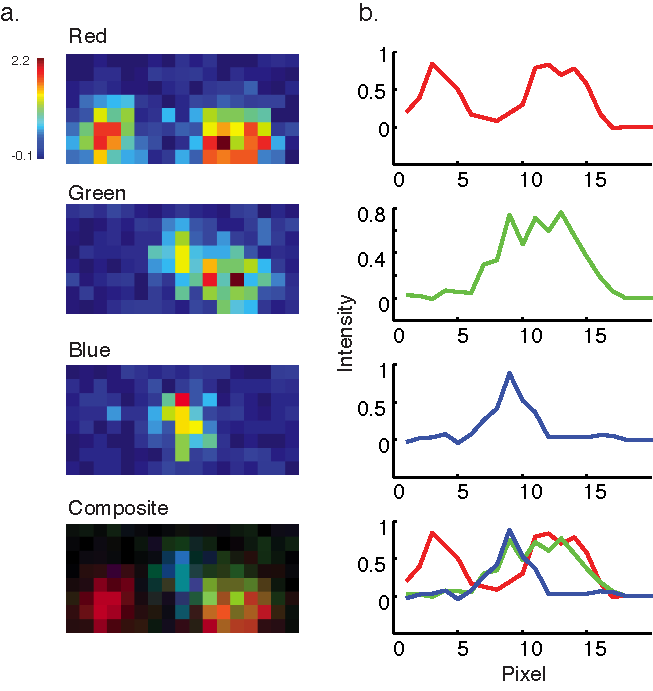
\includegraphics[width=\textwidth]{figures/fullpage}
%\caption[Short figure name.]{This is a full page figure using the FPfigure command. It takes up the whole page and the caption appears on the preceding page. Its useful for large figures. Harvard's rules about full page figures are tricky, but you don't have to worry about it because we took care of it for you. For example, the full figure is supposed to have a title in the same style as the caption but without the actual caption. The caption is supposed to appear alone on the preceding page with no other text. You do't have to worry about any of that. We have modified the fltpage package to make it work. This is a lengthy caption and it clearly would not fit on the same page as the figure. Note that you should only use the FPfigure command in instances where the figure really is too large. If the figure is small enough to fit by the caption than it does not produce the desired effect. Good luck with your thesis. I have to keep writing this to make the caption really long. LaTex is a lot of fun. You will enjoy working with it. Good luck on your post doctoral life! I am looking forward to mine. \label{fig:myFullPageFigure}}
 %\end{FPfigure}
 %\afterpage{\clearpage}
\end{comment}
